\documentclass[10pt,a4paper]{article}
\usepackage[utf8]{inputenc}
\usepackage{amsmath}
\usepackage{amsfonts}
\usepackage{graphicx}
\usepackage{amssymb}
\usepackage{textcomp}
\usepackage{todonotes}
\graphicspath{{img/}}
\author{150016853}
\title{%
CS4303 - P4\\
MorphZone}
\begin{document}

\maketitle

\section{Overview}

A specification has been provided based upon a video game pitch provided with the focus of developing a technically challenging game with novel elements providing a unique playing experience.

Evaluation has been performed with usability tests executed.

\section{Design}

The game provided has been named MorphZone. MorphZone is a PvP, 2D, physics-based, side-on arena shooter with an emphasis on movement tech.

\section{Play Environment}

The gameplay environment is a bounded physical arena. The arena being bounded by walls or destroyer beams. All entities within this environment are collidable. Objects are either static elements restricting player position or non-static player entities/power-ups. Static elements are either damaging laser walls or non-damaging standard walls. Non-static entities are one of a player character model or a power-up.


\begin{figure}[!h]
\centering
  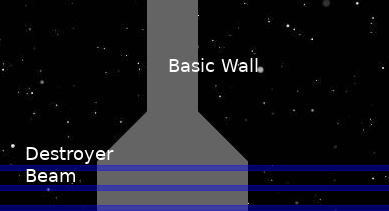
\includegraphics[width=\linewidth]{map_elements.png}
  \caption{Example Map Elements.}
  \label{fig:boat1}
\end{figure}

\subsubsection{Power-ups}

Power ups spawn from a variety of locations around each map. They fall until hitting the ground, where they will remain until either picked up by a player of another force acts on them.

Power ups are of one of two types - weapon or health. Health power ups marginally increase the user health and weapon power ups change the current firing mode of the collecting player. As players collect weapons the weapon type they have collected is highlighted on screen.

\begin{figure}[!h]
\centering
  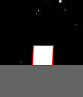
\includegraphics{health_powerup.png}
  \caption{Health Powerup.}
  \label{fig:boat1}
\end{figure}

\begin{figure}[!h]
\centering
  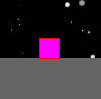
\includegraphics{weapon_powerup.png}
  \caption{Weapon Powerup.}
  \label{fig:boat1}
\end{figure}

\section{Player Entities}

\subsection{Movement}

Players may control their movement in this environment using three movement mechanics. 

A boosting mode has been included as the default movement mode. Users may move apply forces to their player in the direction of their orientation and rotate their model to change orientation. This is limited by a damping system on both linear and rotational velocity. These decision provide a relatively weighty movement feeling, hence facilitating the existence of alternate movement opportunities. When in booting mode the player's elasticity is low. Collisions as such do not result in much bounce on the part of the player.

A tethering mode is available for movement tech. In tethering movement a player may attach a tether to static perpendicular to their orientation. This tether limits their position to within the radius at initial attachment, providing circular movement to the player. The tether is rigid at it's furthest extend but players may move to distances smaller than the radius from the tether location. Whilst in tether mode shadow outlines of the firing line that any tethers they fire would reach are highlighted. This provides a firing guideline for players when tethered. When players are in tether mode their collisions are 50\% elastic. As such they will bounce a great deal more than the other movement options.

A dropper mode has been provided. When activated the player shall experience sudden slowdown, briefly float in the air before plummeting with a massive boost towards the lower portion of the environment. This boost is not subject to any player control and shall only end when the player changes movement mode. The x velocity in this mode is severely damped, making movement almost exclusively in the y direction.

Player characters are restricted by collision hit boxes of entities in the environment. In colliding with entities their character shall be repulsed and, given the direction and location of collision will experience rotational impacts, reducing the controllability of the player.

\subsection{Damage}

Damage in this game is done exclusively through collisions. Collisions of two contact points between a player model and a damaging object above a certain contact velocity shall reduce the player character's health relative to the velocity they collided. This creates a dynamic where control over movement is a primary focus of the learning curve of the game. Understanding the limitations and benefits on each movement tech allows the player to mitigate damage they would otherwise take. Notable examples include that when in tether mode the player's collision damage is reduced by 50\%, allowing transitions to it to reduce collision consequences, though in conjunction with the increased elasticity also increases the likelihood a player will bounce into another collision at high speeds as well as having less predictable movement. The decreased damage however also facilitates more liberal use of the tethering mechanics, with collisions as a consequence of a mis-tether being less punishing, again encouraging their use.

\subsection{Combat}

\subsubsection{Damage Sources}

Combat is done primarily through use of hitscan lasers. Contact with a mobile object adds a large force to the objects at the point of contact, propelling it through the world space. Contact with a player does not do damage to them, instead any damage the player experiences will be as a consequence of collisions with objects which are capable of causing damage. This include walls or destroyer beams (distinct objects from firing lasers).

Destroyer beams, when collided with, cause immediate destruction of the player with which contact occurs.

\subsubsection{Lasers}

Lasers can be fired in variety of modes. These modes are accessed via collecting power-ups which spawn around the map. When a power up is collected the player may exclusively use this mode of fire until they collect another power-up. As lasers are fired a cooldown is initiated during which players may not fire. Once the cooldown expires they may fire again.

Laser power-ups focus on a trade-off of range, force magnitude, number of lasers, lasers spread and cooldown influencing fire rate, damage potential and the ease of use. Four laser types have been provided: standard, machine gun, shotgun and MegaLaser. The standard laser being a single, max range, moderate cool down, moderate force strength laser; the machine gun laser being an automatic, short range, very fast cooldown, low strength laser; the shotgun being multiple very short range, moderate cooldown, moderate strength lasers with a wide spread and the MegaLaser  being multiple, max range, large cool down, high strength lasers with a very tight spread.

\subsubsection{Other Combat}

Damage can be facilitated via other means of colliding opponents. Two players colliding can cause damage to players and push them in directions so in scenarios where damage with a laser is impractical or risky, hitting a player with the player ship can be a useful tool.

Players ability to push opponents also allows for alternate damage. By pushing players via collisions into other objects, such as the walls or destroyer beams one can cause additional damage.

\subsection{Game Rules}

Games are played between two player-controlled entities. Games are played out until 1 or less players is not destroyed. If a player remains they are the winner, otherwise the game is considered a draw. Due to the fast paced, dangerous play environment, a timer did not seem necessary to prevent campy play. Players may immediately reset the world after game over.

\section{Maps}

Players may set the map type as well as the types of walls present, selecting between four maps of varying obstacle layouts as well as selecting from one of four obstacle types: Floored, floorless, floorless/topless and ``?!?!?". In floored no destructor beams are placed and all walls are plain. In floorless, the bottom walls is replaced with a destructor beam, in floorless/topless the bottom and top walls are replaced with destructor beams and in ``?!?!?" all walls are replaced with destructor beams. In selecting a map, one may use any combination of map and wall layout.

On floored maps, small ramps have been placed around the floors. This is done to avoid players getting stuck on the floor should they crash, instead being able to launch themselves skyward. One of the consequences of making the mistake of getting stuck on the floor is that the collision with the ramp if done too quickly will cause damage to the player.

The maps provided include a variety of objects designed to allow the user to tether off them.

\section{Distinctions From Pitch}

The game provided reflects the spirit of the original game, providing a physics based environment with a variety of interesting movement techs which define the way that the user interacts with other players in combat but with some fairly significant distinctions. In the original vision of the game the player's primary combat would be via projectile damage, with the velocity of the projectile influencing the damage the player would take. However it was found that due to limits on the discrete physics engine that has been built that small projectiles in a fast paced environment had very shaky collision detection diminishing the enjoyability of the game. Instead hitscan weapons were found to be fare more consistent, given the lack of reliance on discrete collision. The spirit of the collision damage has been maintained though, with the damage still being a consequence of collisions, rather than hit damage.


\section{Context}

RocketsRocketsRockets (RRR) is a game which features similar elements to this game. With a similar game 2D game environment and a physics based movement system. It features fast-paced gameplay with a variety of different weapon types. Some of the primary differences include the types of weapons, with RRR using a projectile based game environment compared to the hitscan system used in MorphZone. RRR uses collisions with weapons as the damage source of players as well as using a life based system for establishing victory or loss. On top of this the environments are often far more open with no environment hazards to be sources of damage. It's also worth noting the keyboard controls in RRR use discreet directions for keyboard controls, where pressing a key pointing the player in that direction and accelerates them in that direction compared to the more steering based movement used in this game.

A game that more closely aligns to the boosting movement of the player in MorphZone would be LuftRausers, a 2D shoot 'em up. In luftrausers turning on keyboard controls is divided into rotation and thrusting, as in morphzone. However the rotational speed in this game is far faster. Creating an extremely mobile movement tech for the player, whereas the boosting in this game is supposed to be an incomplete movement tech, instead being complemented by other movements. It is also worth noting luftrauser uses little physics based collision response with most collisions being predefined interactions e.g. lose health, with not physics implications for the player. On top of this the game is a PvE game, with no multiplayer interactions.

There are a wide variety of games that employ tether and swinging mechanics in gameplay with major popular examples including games like Spider-Man 2's web-swinging mechanic or the Worms series games' grappling hook. This game aligns most closely to the worms series in terms of the feel of the grappling hook, given the 2D environment however with some distinctions. Notably that worms is a far slower paced game, being turn-based, as such the swinging mechanics are often used more for methodical, slow, movement in rounds - additionally worms tethers are retractable/extendable and collide with the environment they're present in, whereas in MorphZone they are fixed length and can pass through other objects. It's also worth noting the difference in the game environments presents the fact that swinging in MorphZone is not constrained by the y axis the player operates in, not only being useful, but accessibly useable to swing from any position round an object to any other point relative to them, given the swing is within the radius of the tether and the player does not collide with an object.

\subsection{GameUI}

A UI during gameplay highlights player health and the charge rate on their current weapon.

\begin{figure}[!h]
\centering
  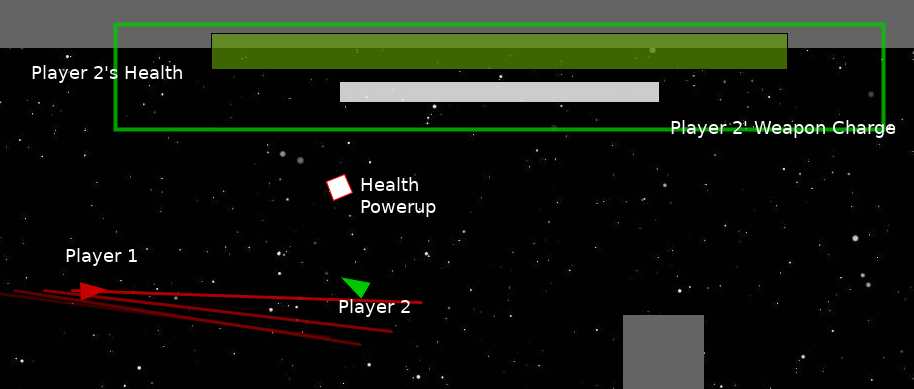
\includegraphics[width=\linewidth]{environment_screen.png}
  \caption{Example UI and Gameplay Visuals.}
  \label{fig:boat1}
\end{figure}

\section{Testing}

Testing was performed primarily with other students in the CS4303 module, though also some outwith. Play was performed across all maps exploring the various movement and combat options for several hours. Multiple issues were found as a result which remain in the game.

\subsection{Known Technical Issues}

\begin{itemize}
\item Certain collisions when tethered cause the player to clip through the wall for brief frames
\item The ``?!?!?!" map is prone to cause FPS drops causing slowdown to the physics engine.
\end{itemize}

Two evaluations were performed. Two extended play sessions with me playing with them and one extended play session with several players and a play guide with a basic early tutorial from me. Requests were made for the first extended play session to provide a written review of their opinions of the game, and in the second, unsupervised play session it was encouraged for the players to voice their thoughts as they played the game and I would note their issues as they were presented.

\subsection{Popular Elements}

The feedback received typically highlighted that the movement was enjoyable to use and that the physics engine combination with the damage system in place was satisfying and enjoyable to use, providing a deal of catharsis. The fast-paced and risky elements were also noted to increase the tension that built to the satisfying moments of success or loss. Players often found the slopes on the ground were fun to ramp off of, highlighting that it complemented the movement.

\subsection{Constructive Criticism}

Users' criticisms was often linked to the combination of the movement mechanics in conjunction with combat system in place, making movement and firing feel slow and cumbersome. This in combination with a high gravity setting made it a chore to move and still attempt to shoot at opponents. This is an interesting point which highlights an interesting design decision to be made. As a direct result the gravity level has been decreased, making movement a lot lighter for the player.

Some players noted the machine gun was disproportionately weak, not firing regular enough to get the benefits of it and not strong enough to reward that it was still hard to hit, as such the firing rate of the machine gun was increased and power marginally increased.

A distinction between evaluation in the groups was that some of the unsupervised group spoke of how the aiming with the laser rifle could be difficult, whereas the supervised group appeared to find the laser rifle aiming suitable. This is again a point where balance is a focus in development. A targeting reticule could be include for players, with a faint outline highlighting the direction of fire at any one point in game so they're aware of where their shot would hit if they were to fire. My only concern with implementing this would be that one would potentially make it too easy to hit opponents, a consequence of having hitscan. Were this to be implemented I believe it would require rebalancing some of the weapons, in particular the laser rifle. 

Players across all groups struggled early on to understand the tethering system worked. The supervised group picked it up fairly quickly, however still seemed uncomfortable using it fluidly. The supervised group struggled regularly.

Players expressed that they found the turning circle too wide when playing in the booster mode, though these issues were reduced as gravity was reduced and as they became accustomed to the movement tech, aligning well with the spirit of the design of the system.

I believe the root of a lot of the distinctions between the groups is that the mechanics could be difficult to learn without sufficient tutoring. As such a more in-depth tutorial system should be implemented into the game, allowing players the time to learn how each element works.

In initial design the tether mode model was direction-less in shape but with orientation in the physics engine and the user control scheme. Players found this confusing, since then a point has been added to the model to highlight the direction of orientation.

\subsection{Personal Observations And Summary}

In watching players from both sets of evaluating groups it became apparent that the groups with myself teaching them came away with overwhelmingly far more positive positions on the game, and, from observation, utilised the movement mechanics far more often and in more interesting ways. Given this, in combination with comments from the unsupervised group's criticism that the movement mechanics controls were confusing and difficulty to use it seems like a priority would be in re-designing the controls of the movement section and including a tutorial mode which provides example scenarios highlighting how the movement mechanics can be integrated into gameplay.

This being said the points the players enjoyed were the fundamental elements that the focus of development was on, with fast movement tech and cathartic physics based combat being highlights of player experience.

The maps provided kept the players interested, though players seemed to enjoy the more destroyer beam focussed map layouts, partially because it complemented high octane, risky play.

\subsection{Next Steps}

I see the primary overarching issues in the game as tied to players not being able to fully utilise the movement techniques that have been implemented. The main components of this being the inability to use the tether mechanics, as such relying on the more typically familiar boosting mechanics, which was designed with the considerations of the tethering mechanic in mind. As such I see a priority in refining the control scheme of the tethering and exposing players to the mechanics built in.

I see the priorities for development in MorphZone focussing on giving users access to a better understanding of and better access to player control and the nuances of combat. The evaluation to me highlights that players typically understood the mechanics involved with relative ease when tutored - with the exception of tethering, which came more slowly - whereas without struggled with lots of the mechanics.

I believe this being said an alternate control scheme on a console controller could be more appropriate for the design of the base game, providing omnidirectional control schemes for tethering.

\begin{thebibliography}{9}
 
\bibitem{rocketsrocketsrockets} 
RocketsRocketsRockets, Radial Games
\\\texttt{https://rocketsrocketsrockets.com/}
Accessed 1/12/2018

\bibitem{luftrausers}
Luftrausers, Vlambeer, Developer Digital
\\\texttt{http://luftrausers.com/}
Accessed 1/12/2018

\bibitem{spiderman}
Spider-Man 2 (Video Game) - Wikipedia
\\\texttt{https://en.wikipedia.org/wiki/Spider-Man\_2\_(video\_game)}
Accessed 1/12/2018

\bibitem{worms}
Worms Series - Wikipedia
\\\texttt{https://en.wikipedia.org/wiki/Worms\_(series)}
Accessed 1/12/2018
\end{thebibliography}

\end{document}